\documentclass{article}
\usepackage{hyperref}
\usepackage[utf8]{inputenc}
\usepackage{wrapfig}
\usepackage{amsmath}
\usepackage{amsthm}
\usepackage{amssymb}
\usepackage[tmargin=1in,bmargin=1in]{geometry}
\usepackage{subcaption}
\usepackage{graphicx}
\usepackage{latexsym}
\usepackage{pdfsync}
\usepackage[boxed]{algorithm}
\usepackage{algpseudocode}
\usepackage{multirow}
\usepackage{rotating}
\usepackage{color}
\usepackage{caption}
\usepackage{url}
\usepackage{diagbox}

\usepackage{fancyvrb}
\usepackage{listings}

\hypersetup{
    colorlinks=true,      		% false: boxed links; true: colored links
    linkcolor=blue,       		% color of internal links
    citecolor=blue,       		% color of links to bibliography
    filecolor=black,      		% color of file links
    urlcolor=red,       		% color of external links
    bookmarks=false,
    pdffitwindow=true,
    pdfpagelayout=SinglePage
}

\newcommand{\etal}{\textit{et al.\ }}
\newcommand{\pd}[2]{\frac{\partial #1}{\partial #2}}
\newcommand{\mbf}[1]{\mathbf{#1}}
\newcommand{\vect}[1]{\underline{\boldsymbol{#1}}}
\newcommand{\tensor}[1]{\underline{\underline{\boldsymbol{#1}}}}
\newcommand{\pest}{\texttt{p4est}}
\newcommand{\caslpest}{\texttt{casl\_p4est}}
\newcommand{\ttt}[1]{\texttt{#1}}
\newcommand{\figb}{\begin{figure}[htbp]\begin{center}}
\newcommand{\fige}{\end{center}\end{figure}}

%%%%%%%%%%%%%%%%%%%%%%%%%%%%%%%%%%%%%%%%%%%%%%%%%%%%%%%%%%%%%%%%%%%%%%%%%%%%%%%%%%%%%%%%%%%%%%%%
%%%%%%%%%%%%%%%%%%%%%%%%%%%%%%%%%%%%%%%%%%%%%%%%%%%%%%%%%%%%%%%%%%%%%%%%%%%%%%%%%%%%%%%%%%%%%%%%
%%%%%%%%%%%%%%%%%%%%%%%%%%%%%%%%%%%%%%%%%%%%%%%%%%%%%%%%%%%%%%%%%%%%%%%%%%%%%%%%%%%%%%%%%%%%%%%%
%%%%%%%%%%%%%%%%%%%%%%%%%%%%%%%%%%%%%%%%%%%%%%%%%%%%%%%%%%%%%%%%%%%%%%%%%%%%%%%%%%%%%%%%%%%%%%%%

\makeindex

\begin{document}

\title{User manual for \texttt{casl\_p4est}}

\author{arthur guittet}

\maketitle

\tableofcontents

\section{Installation}

\subsection{Access to Stampede and Comet}

The first step is to create an account on the XSEDE website (www.xsede.org). After that, the account can be added to an active XSEDE grant by the corresponding PI and the resources available through that allocation can be activated. They need to be activated one by one, for instance if both Stampede and Comet are part of the allocation, each of them needs to be activated separately for the specific user.

Once the access is granted, the login nodes of the clusters can be accessed through ssh with the following commands,
\begin{Verbatim}[frame=single]
ssh username@stampede.tacc.utexas.edu
ssh username@comet.sdsc.edu
\end{Verbatim}
The password is the XSEDE password. Note that when updating the password on XSEDE, several minutes can be required for the update to be propagated to the supercomputers. For ease of access, the following information about an ssh server can be added in \texttt{.ssh/config} (for unix systems)
\begin{Verbatim}[frame=single]
Host stampede
Hostname stampede.tacc.utexas.edu
User username
\end{Verbatim}
A different name can be chosen for the \texttt{Host} part. The supercomputer can then be accessed with
\begin{Verbatim}[frame=single]
ssh stampede
\end{Verbatim}

To transfer files from and to a supercomputer, use the ``scp" or ``rsync" commands for small file, and ``globus" for big transfers between supercomputers (checkout www.globus.org). The documentation for Stampede can be found online on the Texas Advanced Computing Center website, at https://portal.tacc.utexas.edu/user-guides/stampede, and is very well written. The documentation for Comet is not as good ... but they work very similarly.

\subsection{Installing \texttt{p4est}}

The \texttt{p4est} library can be installed from a tarball or directly from the git repository. Some bugs have been fixed and numerous features added since the 1.1 version, and using the git repository is recommended. Start by cloning the repository with
\begin{Verbatim}[frame=single]
git clone https://github.com/cburstedde/p4est.git path_to_local_git_folder
\end{Verbatim}
In the folder created (replace ``path\_to\_local\_git\_folder" with you choice), run
\begin{Verbatim}[frame=single]
git submodule init && git submodule update
\end{Verbatim}
to initialize the \texttt{sc} submodule on which \texttt{p4est} depends. A memory alignment bug was fixed recently, and the branch with the corresponding fix must be selected by
\begin{Verbatim}[frame=single]
git checkout fix-memalign
\end{Verbatim}
in both the main git folder and the ``sc" sub-folder. You then need to run
\begin{Verbatim}[frame=single]
./bootstrap
\end{Verbatim}
from the git folder, followed by the configure command with your choice of option. For a release version, use
\begin{Verbatim}[frame=single]
./configure --prefix=/path/to/install/folder --enable-mpi --without-blas
--enable-shared --enable-memalign=16 CFLAGS=-O2 CPPFLAGS=-O2 FCFLAGS=-O2
\end{Verbatim}
If building for debug, the run
\begin{Verbatim}[frame=single]
./configure --prefix=/path/to/install/folder --enable-mpi --without-blas
--enable-shared --enable-debug --enable-memalign=16 CFLAGS="-O0 -g"
CPPFLAGS="-O0 -g" FCFLAGS="-O0 -g"
\end{Verbatim}
Note that you must have mpi installed and in the PATH. The default install folder (it should be something like ``/usr/lib/p4est") can also be selected by omitting the ``prefix" option. The \texttt{p4est} library can no be built and installed by running
\begin{Verbatim}[frame=single]
./make && ./make install
\end{Verbatim}

The \texttt{casl\_p4est} library also requires \texttt{Petsc}, which is available on the public repositories if running Linux Mint or Ubuntu. Otherwise, you can install it by following the instructions from the \texttt{Petsc} website (https://www.mcs.anl.gov/petsc/). Here are the flags I use if the package is not available on a public repository
\begin{Verbatim}[frame=single]
./configure --download-fblaslapack --download-hypre=1
--prefix=/path/to/install/dir --with-debugging=0 --with-mpi-dir=/path/to/mpi/dir
--with-shared-libraries=1 COPTFLAGS="-O2" CXXOPTFLAGS="-O2" FOPTFLAGS="-O2"
\end{Verbatim}

On Stampede and Comet, you can load the \texttt{Petsc} module with the module manager, by running
\begin{Verbatim}[frame=single]
module load petsc
\end{Verbatim}
The \texttt{p4est} library is also available as a module on Stampede, however it's the 1.1 version that does not have some of the new features and bug fixes that are needed by \texttt{casl\_p4est}.

\subsection{Installing \texttt{casl\_p4est}}

The first step is to create a bitbucket account (at bitbucket.org) and ask someone with admin rights to add you to the git repository. Once this is done, you can clone the repository by running
\begin{Verbatim}[frame=single]
git clone https://username@bitbucket.org/cburstedde/casl_p4est.git local_folder
\end{Verbatim}
where ``username" is your bitbucket username and ``local\_folder" is the path to the folder where the library is to be installed. You can use git through the command line or with a Graphical User Interface. I personally recommend SmartGit.

\subsection{Compiling against the \texttt{casl\_p4est} library}

A sample \texttt{Makefile} and a sample \texttt{project.pro} file are located in the ``doc/casl\_p4est\_manual" folder. The general things you need in you \texttt{Makefile} are
\begin{itemize}
\item include the headers for the \texttt{p4est} library and path to the compiled library for the linker
\begin{Verbatim}[frame=single]
INCPATH += -I/path/to/the/p4est/install/include
LIBS += -Wl,-rpath,/path/to/the/p4est/install/lib
	-L/path/to/the/p4est/install/lib -lp4est -lsc
\end{Verbatim}
\item include the headers for the \texttt{Petsc} library and path to the compiled library for the linker. Depending on the system, the PETSC\_DIR might already be set as an environment variable, it is for instance the case on Stampede.
\begin{Verbatim}[frame=single]
INCPATH += -I/path/to/the/petsc/install/include
LIBS += -Wl,-rpath,/path/to/the/petsc/install/lib
	-L/path/to/the/petsc/install/lib -lpetsc
\end{Verbatim}
\item include the headers for the \texttt{Petsc} library and path to the compiled library for the linker. Depending on the system, the PETSC\_DIR might already be set as an environment variable, it is for instance the case on Stampede.
\begin{Verbatim}[frame=single]
INCPATH += -I/path/to/the/casl/p4est/library
\end{Verbatim}
\end{itemize}

\section{Using the \texttt{p4est} library}

The following sections contain information about the \texttt{p4est} data structures and how to use them, including samples of code.

\subsection{Forests of Octrees and parallelization}

The \pest library works with forests of Octrees, that is a collection of Octrees rooted in a shared macromesh. The macromesh can be complicated, but for the \caslpest we limit ourselves to Cartesian macromeshes. This can be changed in the future if needed. The first step is therefore to declare a macromesh, with
\begin{Verbatim}[frame=single]
my_p4est_brick_t brick;
p4est_connectivity_t *connectivity = my_p4est_brick_new(nx, ny, nz,
				xm, xM, ym, yM, zm, zM, &brick, px, py, pz);
\end{Verbatim}
with \ttt{nx}, \ttt{ny} and \ttt{nz} are the dimensions of the macromesh. For instance, setting those to 2 will generate a 2x2x2 macromesh, i.e. the framework for a forest of 8 Octrees. The other parameters are the physical dimensions of the domain and the periodicity information. Every process knows about the macromesh, it is a shared information.

The forest can now be created and the Octrees refined, for example with a level-set function \ttt{LS} defined as a CF\_3 (Continuous Function in $\mathbb{R}^3$, or CF\_2 in 2d), with
\begin{Verbatim}[frame=single]
p4est_t *p4est = my_p4est_new(mpicomm, connectivity, 0, NULL, NULL);
splitting_criteria_cf_t criteria(lmin, lmax, &LS, 1.2);
p4est->user_pointer = (void*)(&criteria);
for(int lvl=0; lvl<lmax; ++lvl)
{
	my_p4est_refine(p4est, P4EST_FALSE, refine_levelset_cf, NULL);
	my_p4est_partition(p4est, P4EST_FALSE, NULL);
}
\end{Verbatim}
with \ttt{mpicomm} the mpi communicator to use, \ttt{lmin} and \ttt{lmax} the min and max level of each Octree, and \ttt{1.2} the Lipschitz constant for the level-set function (choosen conservatively to be larger than 1 here). The refinement is done within a loop because initially the macromesh is distributed across the processes evenly. This means that a 1x1x1 macromesh will be attributed to a single process, even if running 1024 mpi tasks. Conversely, a 2x2x2 macromesh with 4 processes will result in 2 blocks per process.

The forest is partitioned across processes by linearizing the trees, i.e. building an array of the leaves ordered by a particular procedure based on a space-filling curve. \ttt{p4est} uses the Z-ordering, or Morton ordering. Though alternatives exist (Hilbert curve for instance), their performances are similar to the Z-curve. The array is then distributed evenly across the processes. Figure \ref{fig::zcurve} illustrates the process.
\figb
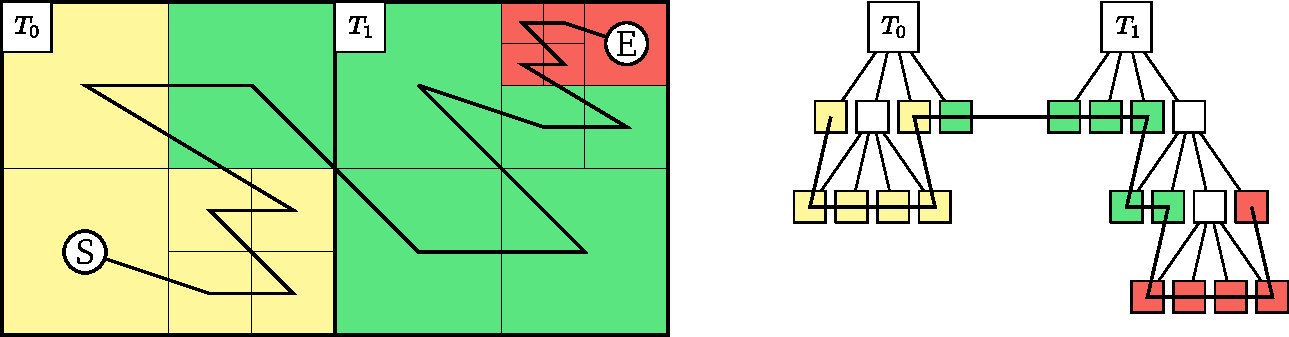
\includegraphics[width=.9\textwidth]{figures/p4est_zcurve.pdf}
\caption{Illustration of the Z-curve ordering and of the partitioning process for a forest of 2 Octrees (macromesh 2x1) and for 3 mpi processes.} \label{fig::zcurve}
\fige


\subsection{Organization of the quadrants}

The forest is now ready for use if the algorithm is based on cell-centered data. Each process knows about its local chunk of the quadrants array, stored inside the local tree structures. The number of quadrants owned by a process is given by
\begin{Verbatim}[frame=single]
p4est->local_num_quadrants
\end{Verbatim}
while the entire forest contains
\begin{Verbatim}[frame=single]
p4est->global_num_quadrants
\end{Verbatim}
Each chunk of the local quadrants belongs to a tree, and thanks to the Z-curve property the values are contiguous. Each tree stores the index at which its quadrants start in the local ordering in
\begin{Verbatim}[frame=single]
tree->quadrants_offset
\end{Verbatim}
\figb
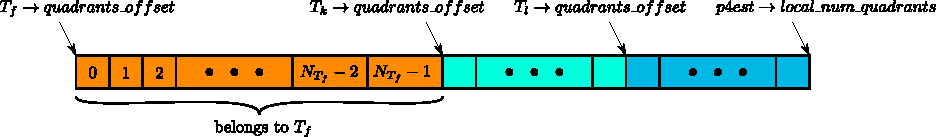
\includegraphics[width=\textwidth]{figures/quadrants.pdf}
\caption{Representation of the quadrants data structure. $T_f$ is the first local tree for the current mpi process, $T_l$ is the last local tree, and $N_{T_f}$ is the number of local quadrants located in tree $T_f$, i.e.\ $T_f \rightarrow \texttt{quadrants} \rightarrow  \texttt{elem\_count}$.} \label{fig::quadrants}
\fige
Figure \ref{fig::quadrants} summarizes the \ttt{quadrants} structure, and the code structure for accessing the quadrants information is
\begin{Verbatim}[frame=single]
for(p4est_topidx_t tree_idx=p4est->first_local_tree;
	tree_idx<=p4est->last_local_tree;
	++tree_idx)
{
  p4est_tree_t *tree = (p4est_tree_t*)sc_array_index(p4est->trees, tree_idx);
  for(size_t q=0; q<tree->quadrants.elem_count; ++q)
  {
    p4est_locidx_t quad_idx = q+tree->quadrants_offset;
    p4est_quadrant_t *quad =
    		(p4est_quadrant_t*)sc_array_index(&tree->quadrants, q);
  }
}
\end{Verbatim}
Here \ttt{quad\_idx} is the index of the quadrant in the local ordering, and \ttt{q} is the index of the quadrant in the local tree. The global index of a local quadrant can be obtained by adding the global offset of its owning process to its index
\begin{Verbatim}[frame=single]
p4est_gloidx_t gloidx = quad_idx + p4est->global_first_quadrant[p4est->mpirank];
\end{Verbatim}

\subsection{The ghost quadrants data structure}

So far, each process only knows about its local information. The \texttt{p4est\_ghost\_t} gives access to a layer of ghost cells around a process. The structure can be initialized with
\begin{Verbatim}[frame=single]
p4est_ghost_t *ghost = my_p4est_ghost_new(p4est, P4EST_CONNECT_FULL);
\end{Verbatim}
\ttt{P4EST\_CONNECT\_FULL} indicates that the ghost neighbors are gathered across faces, edges and corners. This constructs the structure for a ghost layer of depth one. The ghost layer can be expanded with
\begin{Verbatim}[frame=single]
my_p4est_ghost_expand(p4est, ghost);
\end{Verbatim}
This results in a ghost layer of depth two. The expand function can be called the desired number of times to build a ghost layer of larger depth.

The ghost data structures contains the array of quadrants in the ghost layer, stored in
\begin{Verbatim}[frame=single]
ghost->ghosts
\end{Verbatim}
and of size
\begin{Verbatim}[frame=single]
ghost->ghosts.elem_count
\end{Verbatim}
One can loop over the ghost directly with
\begin{Verbatim}[frame=single]
for (g = 0; g < ghost->ghosts.elem_count; ++g)
{
      q = (p4est_quadrant_t*)sc_array_index(&ghost->ghosts, g);
}
\end{Verbatim}
The ghost structure also contains the information about the owner of a ghost quadrant and the tree it belongs to. Figure \ref{fig::ghost_quadrants} illustrate the structure of this information.
\figb
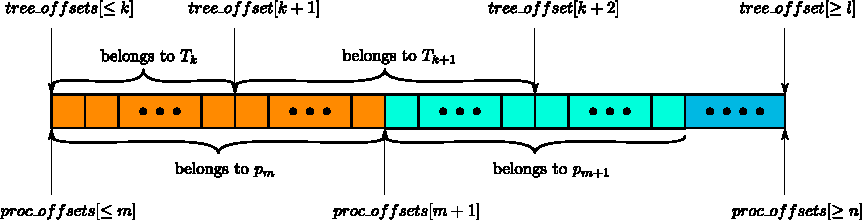
\includegraphics[width=\textwidth]{figures/ghosts.pdf}
\caption{Representation of the ghost layer information. The \ttt{tree\_offsets} arrays and \ttt{proc\_offsets} are members of the \ttt{ghost\_t} data structure. $T_k$ corresponds to the tree of index $k$ and $p_m$ to mpi process of index $m$. For this particular example, the trees of index strictly smaller than $k$ or larger or equal to $l$ are not represented in the ghost layer, and similarly none of the quadrants in the ghost layer belong to a mpi processes with a rank strictly smaller than $m$ or larger or equal to $n$.} \label{fig::ghost_quadrants}
\fige

\subsection{The nodes data structure}

If working on node (i.e.\ vertices) based data, the nodes structure must be initialized. It contains the basic information about the nodes, such as the index of the nodes and the remote information for ghost layer nodes. The nodes structure is initialized by calling
\begin{Verbatim}[frame=single]
p4est_nodes_t *nodes = my_p4est_nodes_new(p4est, ghost);
\end{Verbatim}
The ghost information is optional and can be replaced by \ttt{NULL} if the ghost layer is not used. In the original \ttt{p4est} library, the nodes are organized differently than in \ttt{casl\_p4est}. That is, the ghost nodes for lower ranks are located at the beginning of the nodes array, the ghost nodes for higher ranks are at the end, and the local nodes are in between, starting at \ttt{nodes$\rightarrow$offset\_owned\_indeps}. Furthermore, the hanging nodes are indexed separately.

In \ttt{casl\_p4est}, the nodes are reorganized to match the quadrants organization, thus simplifying the coupling with \ttt{Petsc}.

\subsection{Communications with \texttt{Petsc}}

Most of the communication can be handled with the \ttt{Vec} data type provided by Petsc. The \ttt{Petsc} library is thoroughly documented online. A \ttt{Vec} is an array that can have a ghost chunk. A ghosted array can be created with the data located at the quadrants' center or at the nodes. The nodes code is
\begin{Verbatim}[frame=single]
Vec phi;
VecCreateGhostNodes(p4est, nodes, &phi);
\end{Verbatim}
The actual data stored in the \ttt{Vec} can be accessed by
\begin{Verbatim}[frame=single]
double *phi;
VecGetArray(phi, &phi_p);
for (p4est_locidx_t n = 0; n<nodes->num_owned_indeps; ++n)
{
  (do something with phi_p)
}
VecRestoreArray(phi, &phi_p);
\end{Verbatim}
In the previous code, the pointer \ttt{phi\_p} points to a contiguous array of the local part of the data stored in the \ttt{Vec}. \ttt{Petsc} does not guarantee that the local part and the ghosted part are stored in the same location, and therefore accessing the entire data - including the ghosted part - should be done after getting the local form of the \ttt{Vec}
\begin{Verbatim}[frame=single]
Vec phi_loc;
double *phi_p;
VecGhostGetLocalForm(phi, &phi_loc);
VecGetArray(phi_loc, &phi_p);
for(size_t n=0; n<nodes->indep_nodes.elem_count; ++n)
{
  (do something with phi_p)
}
VecRestoreArray(phi_loc, &phi_p);
VecGhostRestoreLocalForm(phi, &phi_loc);
\end{Verbatim}
In many places in the library, the ghosted values are accessed without first accessing the local form of the \ttt{Vec}, this is a dangerous practice that has worked ... so far.

The ghost values can be synchronized with the remote processes through the \ttt{Petsc} API, thus leading to the general communication layout
\begin{Verbatim}[frame=single]
{ do work for local values shared with other processes }
VecGhostUpdateBegin(phi, INSERT_VALUES, SCATTER_FORWARD);
{ do work for local values not shared with other processes }
VecGhostUpdateEnd(phi, INSERT_VALUES, SCATTER_FORWARD);
\end{Verbatim}

\subsection{Finite differences and local tree reconstruction}

\newpage
\bibliographystyle{abbrv}
\addcontentsline{toc}{section}{\refname}
\bibliography{references}

\end{document}
